\chapter{Termodinâmica das pilhas eletroquímicas}\label{ch:b2:cell-thermodynamics}

Um ônibus a hidrogênio leva uma pilha de algumas centenas de células a
combustível finas. Em cada uma, o hidrogênio e o oxigênio do ar se combinam
em água sem chama, e a energia sai como corrente elétrica. Dois números
governam esse conjunto, e ambos vêm diretamente das tabelas de \omterm{def:b2:reaction-free-energy:gibbs-energy}{energias de
Gibbs}: nenhuma célula pode dar mais que \qty{1.23}{V}, e nenhuma célula a
combustível, por mais perfeita que seja, transforma toda a energia de seu
hidrogênio em trabalho elétrico. Este capítulo liga a tensão de uma pilha à
\omterm{def:b2:reaction-free-energy:gibbs-energy}{energia de Gibbs} de sua reação, demonstra a equação de Nernst usada desde o
volume do 1.º ano e lê entropias e \omterm{def:b2:reaction-enthalpy:reaction-quantity}{entalpias de reação} em um voltímetro e em
um termômetro.

\begin{recall}
O volume do 1.º ano: pilhas, meias-pilhas, ânodo e cátodo, ponte salina,
tensão da pilha, potencial de eletrodo, potencial padrão e eletrodo padrão de
hidrogênio, a equação de Nernst (ali admitida), constantes de equilíbrio a
partir dos potenciais. \Cref{ch:b2:reaction-free-energy}: $\Delta_r G$, $\Delta_r G^\circ$
e $\Delta_r G = \Delta_r G^\circ + RT\ln Q$; o critério de evolução.
\Cref{ch:b2:chemical-potential}: as atividades. O volume escolar: a eletrólise.
\end{recall}

\begin{omfigure}
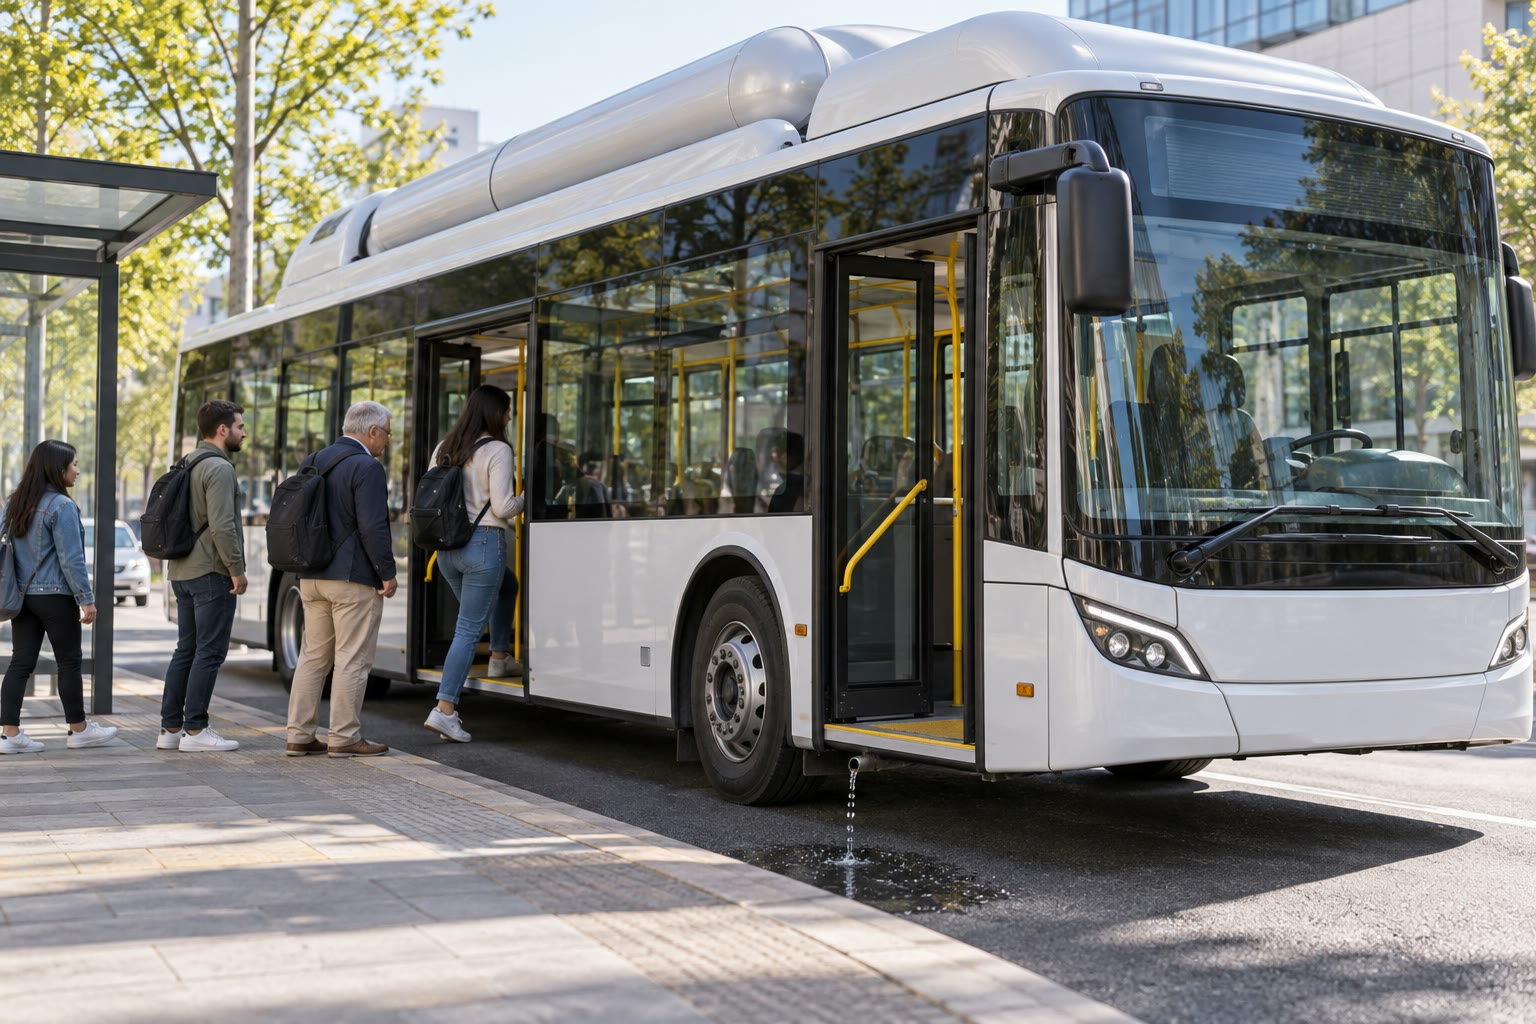
\includegraphics[width=0.62\linewidth]{images/book3/ai/b2-09-fuel-cell-bus.jpg}

{\small Um ônibus a hidrogênio em um ponto: os tanques de hidrogênio ficam sob
a carenagem do teto, e o único escapamento é água, que pinga sob o ônibus.}
\end{omfigure}

\section{Trabalho elétrico e constante de Faraday}

\begin{definition}[Constante de Faraday]\label{def:b2:cell-thermodynamics:faraday}
A \emph{constante de Faraday}\index{constante de Faraday} é a carga elétrica de
um mol de cargas elementares, $F = N_A e = \qty{96485.33}{C/mol}$.
% ledger: const:F
\end{definition}

\begin{proposition}[Carga transportada]\label{prop:b2:cell-thermodynamics:charge}
Se a reação de uma pilha, escrita com $n$ elétrons trocados, avança de
$\Delta\xi$, a carga que circula pelo circuito externo é $Q =
nF\,\Delta\xi$.
\end{proposition}

\begin{proof}
Um avanço $\Delta\xi$ transfere $n\,\Delta\xi$ mols de elétrons do ânodo ao
cátodo pelo fio, cada um de carga $e$ em valor absoluto:
$Q = n\,\Delta\xi\,N_A e$.
\end{proof}

Quando uma carga $Q$ é impulsionada por um circuito por uma tensão $U$, o
trabalho recebido pelo circuito é $QU$. Do ponto de vista da pilha, que
fornece esse trabalho, o trabalho elétrico que ela recebe é
$\delta W_{\text{el}} = -U\,\delta Q = -nFU\,
d\xi$.

\begin{omfigure}
\begin{tikzpicture}[font=\small, >={Stealth}]
  \draw[thick, rounded corners, fill=omDef!8] (0,0) rectangle (3.2,2.2);
  \node[align=center] at (1.6,1.1) {pilha\\ (sistema)\\ reação $d\xi$};
  \draw[->, thick, omThm] (3.2,1.6) -- (5.6,1.6) node[right, align=left] {$\delta W_{\text{el}}$ fornecido\\ $= nFU\,d\xi$};
  \draw[->, thick, omDef] (5.6,0.6) -- (3.2,0.6) node[pos=0, right, align=left] {$\delta Q_{\text{calor}}$ recebido\\ (de qualquer sinal)};
  \draw[<->, thick] (1.6,2.2) -- (1.6,3.0) node[above] {vizinhança a $T$, $p$};
\end{tikzpicture}

{\small Uma pilha como sistema termodinâmico a temperatura e pressão
constantes: ela troca calor com a vizinhança e fornece trabalho elétrico pelo
circuito externo. Com a convenção de sinais da primeira lei (trabalho e calor
recebidos contados positivamente), $\delta W_{\text{el}} = -nFU\,d\xi$.}
\end{omfigure}

\section{A energia de Gibbs da reação de uma pilha}

\begin{theorem}[Trabalho elétrico e energia de Gibbs]\label{thm:b2:cell-thermodynamics:delta-g-nfe}
Uma pilha que funciona a $T$ e $p$ constantes fornece um trabalho elétrico no
máximo igual à diminuição de sua \omterm{def:b2:reaction-free-energy:gibbs-energy}{energia de Gibbs}: para um avanço $d\xi$,
$nFU\,d\xi \leq -\Delta_r G\,d\xi$. Quando ela funciona de modo reversível
(com uma corrente infinitesimal), vale a igualdade, e a tensão da pilha é a
força eletromotriz
\[
  \Delta_r G = -nFE .
\]
\end{theorem}

\begin{proof}
Primeira lei a pressão constante, com o trabalho de pressão separado:
$dH = \delta Q + \delta W_{\text{el}}$. Segunda lei: $dS \geq \delta Q/T$. A
$T$ e $p$ constantes, $dG = dH - T\,dS \leq \delta W_{\text{el}} = -nFU\,d\xi$.
Com $dG = \Delta_r G\,d\xi$, $\Delta_r G\,d\xi \leq -nFU\,d\xi$, isto é,
$nFU\,d\xi \leq -\Delta_r G\,d\xi$. Para uma transformação reversível, a
desigualdade da segunda lei é uma igualdade, e a tensão então medida, sem
corrente, é $E$: $\Delta_r G = -nFE$.
\end{proof}

Uma pilha só pode, portanto, funcionar no sentido direto ($d\xi > 0$,
fornecendo trabalho) se $\Delta_r G <
0$, isto é, $E > 0$, com os polos escolhidos de modo que a reação escrita
vá do ânodo ao cátodo. Uma pilha real, percorrida por uma corrente, fornece
menos trabalho que $-\Delta_r G$: a diferença é dissipada como calor em sua
resistência e em seus eletrodos (\cref{ch:b2:current-potential-curves}).

\begin{example}[A pilha de Daniell]\label{ex:b2:cell-thermodynamics:daniell}
Para \ce{Zn + Cu^2+ -> Zn^2+ + Cu}, $\Delta_r G^\circ = \Delta_f G^\circ(\ce{Zn^2+}) -
\Delta_f G^\circ(\ce{Cu^2+}) = -147.06 - 65.49 = \qty{-212.55}{kJ/mol}$, e $n = 2$:
$E^\circ = 212\,550/(2 \times 96\,485) = \qty{1.10}{V}$, a tensão medida em uma
pilha de Daniell em condições padrão.
% ledger: dfg:Zn2+_ao, dfg:Cu2+_ao, const:F, emf:Daniell
\end{example}

\section{A equação de Nernst e os potenciais padrão}

O volume do 1.º ano admitiu a equação de Nernst; ela agora decorre de
$\Delta_r G = \Delta_r G^\circ + RT\ln Q$.

\begin{theorem}[A equação de Nernst, demonstrada]\label{thm:b2:cell-thermodynamics:nernst-derived}
Para uma semirreação $\alpha\,\mathrm{Ox} + n\,\mathrm e^- \rightleftharpoons
\beta\,\mathrm{Red}$, o potencial do eletrodo à temperatura $T$ é
\[
  E = E^\circ + \frac{RT}{nF}\ln\frac{a_{\mathrm{Ox}}^{\alpha}}{a_{\mathrm{Red}}^{\beta}} ,
\]
em que as atividades incluem as de todas as outras espécies da
semirreação (\ce{H+}, exceto a água), com suas potências estequiométricas.
\end{theorem}

\begin{proof}
O potencial de um eletrodo é a tensão da pilha formada pelo eletrodo padrão
de hidrogênio (ânodo) e por esse eletrodo (cátodo). Sua reação é
\[
  \alpha\,\mathrm{Ox} + \tfrac n2\,\ce{H2} \longrightarrow \beta\,\mathrm{Red} + n\,\ce{H+} ,
\]
cujo quociente de reação, com $a_{\ce{H+}} = 1$ e $p_{\ce{H2}} = p^\circ$ no
eletrodo padrão de hidrogênio, se reduz a $a_{\mathrm{Red}}^\beta/
a_{\mathrm{Ox}}^\alpha$. Pelo \cref{thm:b2:cell-thermodynamics:delta-g-nfe},
$E = -\Delta_r G/(nF) = -\Delta_r G^\circ/(nF) - (RT/nF)\ln Q$; com $E^\circ =
-\Delta_r G^\circ/(nF)$, obtém-se a fórmula. A \qty{298.15}{K}, $RT\ln 10/F =
\qty{0.0592}{V}$.
\end{proof}

\begin{proposition}[Potenciais padrão a partir das energias de Gibbs]\label{prop:b2:cell-thermodynamics:standard-potential}
Com as convenções $\Delta_f G^\circ(\ce{H+}, \text{aq}) = 0$ e
$\Delta_f G^\circ(\ce{H2}, \text{g}) = 0$, o potencial padrão de um par é
$E^\circ = -\Delta_r G^\circ/(nF)$, em que $\Delta_r G^\circ$ é a \omterm{def:b2:reaction-free-energy:gibbs-energy}{energia de
Gibbs} padrão da semirreação escrita como redução, contando-se os elétrons
com \omterm{def:b2:reaction-free-energy:gibbs-energy}{energia de Gibbs} nula.
\end{proposition}

\begin{proof}
Na reação contra o eletrodo de hidrogênio, $\tfrac n2\,\ce{H2}$ e
$n\,\ce{H+}$ não contribuem para $\Delta_r G^\circ$ com essas convenções: a
\omterm{def:b2:reaction-free-energy:gibbs-energy}{energia de Gibbs} padrão da reação da pilha é a da semirreação sozinha.
\end{proof}

\begin{method}[Um potencial padrão a partir das tabelas]\label{met:b2:cell-thermodynamics:e-from-gibbs}
\begin{enumerate}
  \item Escreva a semirreação como redução, balanceada com \ce{H+} e
        \ce{H2O}, com $n$ elétrons.
  \item Calcule $\Delta_r G^\circ = \sum\nu_i\Delta_f G^\circ_i$ (produtos
        positivos), com zero para os elementos, para \ce{H+} e para os elétrons.
  \item $E^\circ = -\Delta_r G^\circ/(nF)$, em volts, com $\Delta_r G^\circ$ em
        joules por mol.
\end{enumerate}
\end{method}

\begin{example}[O eletrodo de cloreto de prata]\label{ex:b2:cell-thermodynamics:agcl}
\ce{AgCl(s) + e- -> Ag(s) + Cl^-}: $\Delta_r G^\circ = -131.228 - (-109.789) =
\qty{-21.439}{kJ/mol}$, $E^\circ = 21\,439/96\,485 = \qty{0.222}{V}$. Seu potencial
depende apenas da atividade do cloreto: em uma solução saturada de cloreto
de potássio, ele é um eletrodo de referência estável.
% ledger: dfg:Cl-_ao, dfg:AgCl_cr
\end{example}

\begin{proposition}[Combinação de potenciais]\label{prop:b2:cell-thermodynamics:combining}
Se uma semirreação (3), com $n_3$ elétrons, é a soma das semirreações (1)
e (2), com $n_1$ e $n_2$ elétrons, então
\[
  n_3E_3^\circ = n_1E_1^\circ + n_2E_2^\circ ;
\]
os próprios potenciais não se somam.
\end{proposition}

\begin{proof}
As \omterm{def:b2:reaction-free-energy:gibbs-energy}{energias de Gibbs} padrão se somam, $\Delta_r G_3^\circ = \Delta_r G_1^\circ + \Delta_r
G_2^\circ$, e os números de elétrons também, $n_3 = n_1 + n_2$. Divida cada $\Delta_r
G^\circ$ por $-F$.
\end{proof}

\begin{example}[O ferro em seus dois estados de oxidação]\label{ex:b2:cell-thermodynamics:iron}
\ce{Fe^3+ + e- -> Fe^2+} tem $E^\circ = (-78.90 + 4.7)/(-96.485) = \qty{0.77}{V}$
e \ce{Fe^2+ + 2e- -> Fe} tem $E^\circ = -78.90/(2 \times 96.485) =
\qty{-0.41}{V}$. Logo, \ce{Fe^3+ + 3e- -> Fe}: $E^\circ = (0.77 - 0.82)/3 =
\qty{-0.02}{V}$, e não a soma dos dois.
% ledger: dfg:Fe2+_ao, dfg:Fe3+_ao
\end{example}

\section{Temperatura, entropia e rendimento de uma célula a combustível}

\begin{definition}[Coeficiente de temperatura]\label{def:b2:cell-thermodynamics:temperature-coefficient}
O \emph{coeficiente de temperatura}\index{coeficiente de temperatura} de uma pilha é
a derivada $(\partial E/\partial T)_p$ de sua força eletromotriz em relação
à temperatura.
\end{definition}

\begin{proposition}[Entropia e entalpia a partir de dados da pilha]\label{prop:b2:cell-thermodynamics:entropy}
Para a reação padrão da pilha,
\[
  \Delta_r S^\circ = nF\,\frac{dE^\circ}{dT}, \qquad
  \Delta_r H^\circ = -nF\Big(E^\circ - T\frac{dE^\circ}{dT}\Big),
\]
e uma pilha que funciona de modo reversível à temperatura $T$ recebe de sua
vizinhança o calor $T\Delta_r S$ por mol de reação.
\end{proposition}

\begin{proof}
$\Delta_r S^\circ = -d\Delta_r G^\circ/dT$ (a partir de $dG = -S\,dT + V\,dp$,
derivada em relação a $\xi$) $= nF\,dE^\circ/dT$; depois, $\Delta_r H^\circ = \Delta_r G^\circ
+ T\Delta_r S^\circ$. Para a transformação reversível, $\delta Q = T\,dS = T\Delta_r S\,
d\xi$.
\end{proof}

\begin{method}[Dos dados da pilha à termodinâmica da reação]\label{met:b2:cell-thermodynamics:cell-data}
\begin{enumerate}
  \item Meça $E$ a várias temperaturas; a inclinação é $dE/dT$.
  \item $\Delta_r G = -nFE$, $\Delta_r S = nF\,dE/dT$, $\Delta_r H = \Delta_r G +
        T\Delta_r S$.
  \item Calor trocado por mol quando a pilha funciona de modo reversível:
        $T\Delta_r S$; quando ela fornece uma corrente sob uma tensão $U < E$,
        o calor liberado é $-\Delta_r H - nFU$ por mol.
\end{enumerate}
\end{method}

Para a pilha hidrogênio--oxigênio que produz água líquida, os valores-chave do
CODATA dão $\Delta_r H^\circ = \qty{-285.83}{kJ/mol}$ e
\[
  \Delta_r S^\circ = 69.95 - 130.68 - \tfrac12 \times 205.15 = \qty{-163.3}{J/(K.mol)} ,
\]
logo $\Delta_r G^\circ = \qty{-237.14}{kJ/mol}$ e $E^\circ = \qty{1.229}{V}$; o
\omterm{def:b2:cell-thermodynamics:temperature-coefficient}{coeficiente de temperatura} é $\Delta_r S^\circ/(2F) = \qty{-0.85}{mV/K}$. Uma
célula a combustível de hidrogênio dá menos tensão a quente do que a frio.
% ledger: dfh:H2O-l, s0:H2O_l, s0:H2_g, s0:O2_g, janafG:H2O_l.298

\begin{omfigure}
\begin{tikzpicture}
\begin{axis}[width=0.48\linewidth, height=5.4cm, xmin=280, xmax=1020,
  ymin=0.95, ymax=1.26, axis x line=bottom, axis y line=left,
  xlabel={$T$ (K)}, ylabel={$E^\circ$ (V)}, tick label style={font=\small},
  label style={font=\small}, title={\small tensão padrão}]
\addplot[omDef, thick, mark=*, mark size=1.2pt] table[x=T, y=E] {figdata/out/bachelor-2-cell-thermodynamics-a-liquid.dat};
\addplot[omThm, thick, mark=*, mark size=1.2pt] table[x=T, y=E] {figdata/out/bachelor-2-cell-thermodynamics-a-gas.dat};
\node[font=\scriptsize, omDef, anchor=north east] at (axis cs:480,1.05) {água líquida};
\node[font=\scriptsize, omThm, anchor=south west] at (axis cs:560,1.12) {vapor d'água};
\end{axis}
\end{tikzpicture}\hfill
\begin{tikzpicture}
\begin{axis}[width=0.48\linewidth, height=5.4cm, xmin=280, xmax=1520,
  ymin=0, ymax=1.0, axis x line=bottom, axis y line=left,
  xlabel={$T$ (K)}, ylabel={rendimento}, tick label style={font=\small},
  label style={font=\small}, title={\small rendimento máximo}]
\addplot[omThm, thick, mark=*, mark size=1.2pt] table[x=T, y=eta] {figdata/out/bachelor-2-cell-thermodynamics-b.dat};
\addplot[black!60, thick, dashed] table[x=T, y=eta] {figdata/out/bachelor-2-cell-thermodynamics-b-carnot.dat};
\node[font=\scriptsize, omThm, anchor=south] at (axis cs:700,0.87) {célula a combustível};
\node[font=\scriptsize, black!70, anchor=north west] at (axis cs:520,0.40) {Carnot, $T_0 = \qty{298}{K}$};
\end{axis}
\end{tikzpicture}

{\small A pilha hidrogênio--oxigênio segundo as tabelas JANAF. À esquerda:
tensão padrão $-\Delta_r G^\circ/(2F)$ com água líquida (até \qty{500}{K},
mantido o líquido em seu estado padrão) e com vapor d'água. À direita:
rendimento máximo $\Delta_r G^\circ/\Delta_r H^\circ$ da célula que produz
vapor, comparado com o rendimento de Carnot de uma máquina térmica que opera
entre $T$ e \qty{298}{K}; a máquina só vence acima de cerca de \qty{1150}{K}.}
% ledger: janafG:H2O_l.298, janafG:H2O_l.300, janafG:H2O_l.400, janafG:H2O_l.500, janafG:H2O.298, janafG:H2O.300, janafG:H2O.400, janafG:H2O.500, janafG:H2O.600, janafG:H2O.700, janafG:H2O.800, janafG:H2O.900, janafG:H2O.1000, janafdfH:H2O_g.300, janafdfH:H2O_g.400, janafdfH:H2O_g.500, janafdfH:H2O_g.600, janafdfH:H2O_g.700, janafdfH:H2O_g.800, janafdfH:H2O_g.900, janafdfH:H2O_g.1000, janafdfH:H2O_g.1100, janafdfH:H2O_g.1300, janafdfH:H2O_g.1500, janafG:H2O.1100, janafG:H2O.1300, janafG:H2O.1500
\end{omfigure}

\begin{definition}[Rendimento termodinâmico de uma célula a combustível]\label{def:b2:cell-thermodynamics:efficiency}
O \emph{rendimento termodinâmico}\index{rendimento termodinamico@rendimento termodinâmico} de uma célula a
combustível é a razão entre o trabalho elétrico que ela fornece e o calor que
seu combustível liberaria por combustão à mesma temperatura, $-\Delta_r H$ por mol.
\end{definition}

\begin{proposition}[Rendimento máximo de uma célula a combustível]\label{prop:b2:cell-thermodynamics:efficiency}
O \omterm{def:b2:cell-thermodynamics:efficiency}{rendimento termodinâmico} de uma célula a combustível é no máximo $\Delta_r G/\Delta_r H$,
atingido quando ela funciona de modo reversível, e igual a $(nFU)/(-\Delta_r H)$
sob uma tensão de trabalho $U$. Ao contrário de uma máquina térmica, ele não é
limitado pelo rendimento de Carnot $1 - T_0/T$.
\end{proposition}

\begin{proof}
Pelo \cref{thm:b2:cell-thermodynamics:delta-g-nfe}, o trabalho por mol é $nFU \leq
-\Delta_r G$; divida por $-\Delta_r H$. A célula converte energia química
diretamente em trabalho a uma única temperatura: nenhum calor é tirado de uma
fonte quente e cedido em parte a uma fonte fria; por isso o limite de Carnot,
que diz respeito a tais ciclos, não se aplica. Seu próprio limite é fixado por
$T\Delta_r S$, o calor que a célula reversível precisa trocar.
\end{proof}

\begin{omfigure}
\begin{tikzpicture}[font=\small, x=0.022cm, y=0.6cm]
  \draw[->] (0,0) -- (320,0) node[right, font=\scriptsize] {\unit{kJ/mol}};
  \foreach \v in {0,100,200,300} \draw (\v,0) -- (\v,-0.12) node[below, font=\scriptsize] {\v};
  \fill[omThm!70] (0,2.2) rectangle (285.83,2.8);
  \node[anchor=west, font=\scriptsize] at (290,2.5) {$-\Delta_r H^\circ = 285.8$: calor de combustão};
  \fill[omDef!70] (0,1.2) rectangle (237.14,1.8);
  \fill[omProp!70] (237.14,1.2) rectangle (285.83,1.8);
  \node[anchor=west, font=\scriptsize] at (290,1.5) {$-\Delta_r G^\circ = 237.1$ de trabalho $+$ $48.7$ de calor};
  \fill[omDef!40] (0,0.2) rectangle (135.1,0.8);
  \fill[omProp!40] (135.1,0.2) rectangle (285.83,0.8);
  \node[anchor=west, font=\scriptsize] at (290,0.5) {a \qty{0.70}{V}: $135.1$ de trabalho $+$ $150.7$ de calor};
\end{tikzpicture}

{\small Para onde vai a energia de um mol de hidrogênio em uma célula a
combustível a \qty{298}{K} (água líquida). Em cima: o calor que uma chama
liberaria. No meio: a célula reversível, que precisa ceder
$-T\Delta_r S^\circ = \qty{48.7}{kJ}$ como calor, qualquer que seja seu
projeto. Embaixo: uma célula real que funciona a \qty{0.70}{V}.}
% ledger: dfh:H2O-l, s0:H2O_l, s0:H2_g, s0:O2_g, const:F
\end{omfigure}

\begin{history}[As leis de Faraday da eletrólise]
\begin{minipage}[t]{0.27\linewidth}
\vspace{0pt}
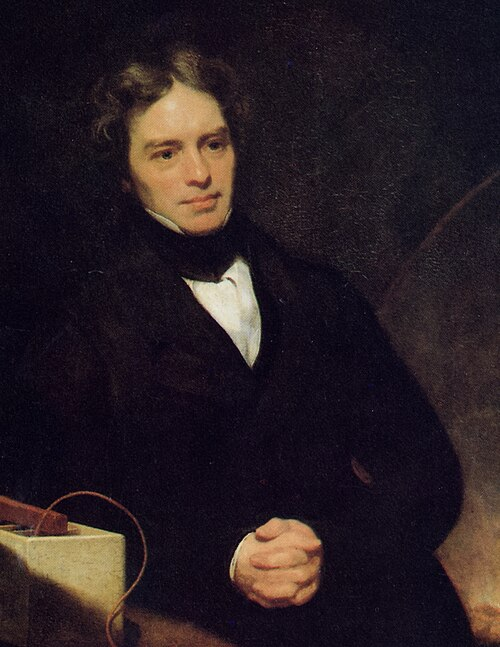
\includegraphics[width=\linewidth]{images/book3/faraday.jpg}
\end{minipage}\hfill
\begin{minipage}[t]{0.69\linewidth}
\vspace{0pt}
Em 1834, Michael Faraday, medindo os produtos de eletrólises com um voltâmetro
de sua própria concepção, enunciou que a massa de uma substância produzida
em um eletrodo é proporcional à quantidade de eletricidade que passou e que,
para uma dada quantidade de eletricidade, as massas de substâncias diferentes
estão na razão de seus equivalentes químicos. Ele cunhou as palavras
eletrodo, ânodo, cátodo, íon, ânion e cátion. A constante que leva seu
nome transforma essas leis em $Q = nF\,\Delta\xi$. (Retrato por Thomas
Phillips, 1842, domínio público, Wikimedia Commons.)
\end{minipage}
\end{history}

\section{Pilhas de concentração}

\begin{definition}[Pilha de concentração]\label{def:b2:cell-thermodynamics:concentration-cell}
Uma \emph{pilha de concentração}\index{pilha de concentracao@pilha de concentração} é formada por
duas meias-pilhas do mesmo par que diferem apenas pela concentração (ou
pela pressão) de uma espécie.
\end{definition}

\begin{proposition}[Tensão de uma pilha de concentração]\label{prop:b2:cell-thermodynamics:concentration-cell}
Dois eletrodos de um metal M mergulhados em soluções de \ce{M^{n+}} de
concentrações $c_1 < c_2$, ligadas por uma ponte salina, dão uma tensão
\[
  U = \frac{RT}{nF}\ln\frac{c_2}{c_1} ,
\]
sendo o polo positivo o lado mais concentrado. A pilha funciona até que as
duas concentrações se igualem.
\end{proposition}

\begin{proof}
Pela equação de Nernst, cada eletrodo tem $E_i = E^\circ + (RT/nF)\ln c_i$
(\omterm{def:b2:chemical-potential:ideal-mixture}{soluções diluídas ideais}); $E^\circ$ se cancela na diferença. A reação é
\ce{M^{n+}}(lado 2) $\to$ \ce{M^{n+}}(lado 1): o metal se deposita no lado
concentrado (cátodo) e se dissolve no lado diluído (ânodo), o que iguala as
concentrações; $\Delta_r G = RT\ln(c_1/c_2) < 0$ até que elas sejam
iguais.
\end{proof}

\begin{omfigure}
\begin{tikzpicture}[font=\small, >={Stealth}]
  \pic at (0,0) {beaker={0.7}{omDef!10}};
  \pic at (3.6,0) {beaker={0.7}{omDef!32}};
  \pic at (-0.3,0.25) {electrode={black!25}};
  \pic at (3.9,0.25) {electrode={black!25}};
  \pic at (0.35,0.55) {saltbridge={2.9}};
  \pic (m) at (1.8,4.3) {meter={V}};
  % common (black) terminal on the anode side, red (+) on the cathode side
  \fill[black] (1.4,4.03) circle (0.065); \fill[red!70!black] (2.2,4.03) circle (0.065);
  \draw[thick] (-0.15,2.65) |- (m-a);
  \draw[thick] (4.05,2.65) |- (m-b);
  \node[anchor=east] at (-0.95,1.0) {\ce{Ag}};
  \node[anchor=west] at (4.45,1.0) {\ce{Ag}};
  \node at (0.25,-0.35) {\ce{Ag+} \qty{0.010}{mol/L}};
  \node at (3.6,-0.35) {\ce{Ag+} \qty{0.10}{mol/L}};
  \node[anchor=east] at (-0.9,2.3) {$-$ ânodo};
  \node[anchor=west] at (4.6,2.3) {cátodo $+$};
  \node[font=\scriptsize] at (-0.1,-0.8) {\ce{Ag -> Ag+ + e-}};
  \node[font=\scriptsize] at (3.7,-0.8) {\ce{Ag+ + e- -> Ag}};
  \node[font=\scriptsize] at (1.8,5.05) {$U = \qty{59}{mV}$};
\end{tikzpicture}

{\small Uma \omterm{def:b2:cell-thermodynamics:concentration-cell}{pilha de concentração} de prata a \qty{25}{\degreeCelsius}. O lado
diluído é o ânodo: a prata se dissolve ali e se deposita no lado concentrado,
até que as duas concentrações sejam iguais. $U = 0.0592\log(0.10/0.010) =
\qty{59}{mV}$.}
\end{omfigure}

O mesmo princípio mede concentrações. Um eletrodo de vidro, cuja fina
membrana separa uma solução de referência da amostra, desenvolve um potencial
de membrana de $(RT/F)\ln 10 = \qty{59}{mV}$ por unidade de diferença de pH a
\qty{25}{\degreeCelsius}: o pHmetro do volume do 1.º ano é uma \omterm{def:b2:cell-thermodynamics:concentration-cell}{pilha de
concentração} para \ce{H+}. Através da membrana de uma célula viva, as
concentrações desiguais de \ce{K+} criam da mesma forma um potencial de
várias dezenas de milivolts.

\section{Exercícios}

\begin{exercise}[$\star$]\label{exo:b2:cell-thermodynamics:1}
A partir de $\Delta_f G^\circ(\ce{H2O}, \text{l}) = \qty{-237.14}{kJ/mol}$, calcule a
tensão padrão da pilha hidrogênio--oxigênio.
\end{exercise}

\begin{exercise}[$\star$]\label{exo:b2:cell-thermodynamics:2}
Uma pilha tem capacidade nominal de \qty{1.0}{A.h}. Calcule a carga que ela
armazena, em coulombs, e a massa de zinco consumida em seu ânodo (\ce{Zn -> Zn^2+ + 2e-}) quando ela
se descarrega completamente.
\end{exercise}

\begin{exercise}[$\star$]\label{exo:b2:cell-thermodynamics:3}
Uma pilha de Daniell fornece \qty{1.10}{V} sem corrente. Calcule $\Delta_r G$ para um
mol de zinco e o trabalho elétrico máximo para \qty{10.0}{g} de zinco.
\end{exercise}

\begin{exercise}[$\star$]\label{exo:b2:cell-thermodynamics:4}
Dois eletrodos de cobre mergulham em soluções de sulfato de cobre(II) de
\qty{1.0e-3}{mol/L} e \qty{0.10}{mol/L}. Calcule a tensão a \qty{25}{\degreeCelsius} e
identifique os polos.
\end{exercise}

\begin{exercise}[$\star\star$]\label{exo:b2:cell-thermodynamics:5}
Uma pilha ($n = 2$) tem $E^\circ = \qty{1.015}{V}$ e $dE^\circ/dT = \qty{-4.0e-4}{V/K}$
a \qty{298}{K} (dados do exercício). Calcule $\Delta_r G^\circ$, $\Delta_r S^\circ$ e
$\Delta_r H^\circ$.
\end{exercise}

\begin{exercise}[$\star\star$]\label{exo:b2:cell-thermodynamics:6}
A pilha do \cref{exo:b2:cell-thermodynamics:5} descarrega um mol de reação
(a) de modo reversível; (b) a \qty{0.90}{V}. Calcule, em cada caso, o trabalho
elétrico e o calor trocado com a vizinhança.
\end{exercise}

\begin{exercise}[$\star\star$]\label{exo:b2:cell-thermodynamics:7}
Calcule $E^\circ(\ce{Fe^3+}/\ce{Fe})$ a partir das \omterm{def:b2:reaction-free-energy:gibbs-energy}{energias de Gibbs} de formação
(\ce{Fe^2+} \qty{-78.90}{kJ/mol}, \ce{Fe^3+} \qty{-4.7}{kJ/mol}) e verifique que ele
é igual a $(E_1^\circ + 2E_2^\circ)/3$.
\end{exercise}

\begin{exercise}[$\star\star$]\label{exo:b2:cell-thermodynamics:8}
Calcule o potencial padrão do par \ce{AgCl}/\ce{Ag} e depois o potencial de um
eletrodo de cloreto de prata mergulhado em cloreto de potássio a
\qty{0.10}{mol/L}.
\end{exercise}

\begin{exercise}[$\star\star$]\label{exo:b2:cell-thermodynamics:9}
As pilhas zinco--ar usam \ce{2Zn + O2 -> 2ZnO} ($\Delta_f G^\circ(\ce{ZnO}) =
\qty{-318.30}{kJ/mol}$). Calcule a tensão padrão e a energia elétrica máxima,
em \unit{kW.h}, por quilograma de zinco.
\end{exercise}

\begin{exercise}[$\star\star\star$]\label{exo:b2:cell-thermodynamics:10}
Uma célula a combustível de metanol direto funciona com \ce{CH3OH(l) + 3/2O2 -> CO2 + 2H2O(l)}. A partir de
$\Delta_f H^\circ$ (\unit{kJ/mol}): \ce{CH3OH(l)} $-239$, \ce{CO2} $-393.51$,
\ce{H2O(l)} $-285.83$; e de $S^\circ$ (\unit{J/(K.mol)}): \ce{CH3OH(l)} 127.2,
\ce{CO2} 213.8, \ce{H2O(l)} 69.95, \ce{O2} 205.15, calcule $n$, $E^\circ$ e o
rendimento máximo.
\end{exercise}

\begin{exercise}[$\star\star\star$]\label{exo:b2:cell-thermodynamics:11}
Uma pilha ($n = 2$) tem $E = \qty{0.500}{V}$ e $dE/dT = \qty{+3.0e-4}{V/K}$ a
\qty{298}{K} (dados do exercício). Mostre que, funcionando de modo reversível,
ela fornece mais trabalho elétrico que $-\Delta_r H$, e explique de onde vem a
energia adicional.
\end{exercise}

\begin{exercise}[$\star\star\star$]\label{exo:b2:cell-thermodynamics:12}
Dois eletrodos de hidrogênio (\qty{1}{bar} de \ce{H2}) mergulham em uma solução
de referência de pH 7.00 e em uma amostra. A tensão é de \qty{0.177}{V} a
\qty{25}{\degreeCelsius}, sendo a referência o polo positivo. Encontre o pH da
amostra e explique por que o resultado não depende de nenhum potencial padrão.
\end{exercise}

\section{Problema: O ônibus a hidrogênio}

\begin{problem}[{Problema de fim de semana --- a tensão padrão da pilha
hidrogênio--oxigênio a partir das energias de Gibbs, seu coeficiente de
temperatura, o rendimento e o calor de uma pilha real e a energia de um
tanque de hidrogênio}]
\label{pb:b2:cell-thermodynamics:1}
Uma pilha de células a combustível tem 400 células em série, cada uma com uma
membrana de troca de prótons (eletrólito ácido). Dados a \qty{298.15}{K} (CODATA, JANAF):
$\Delta_f H^\circ(\ce{H2O}, \text{l}) = \qty{-285.83}{kJ/mol}$, $\Delta_f
G^\circ(\ce{H2O}, \text{l}) = \qty{-237.14}{kJ/mol}$, $\Delta_f G^\circ(\ce{H2O},
\text{g}) = \qty{-228.58}{kJ/mol}$; $S^\circ$ (\unit{J/(K.mol)}): \ce{H2O(l)} 69.95,
\ce{H2} 130.68, \ce{O2} 205.15. $F = \qty{96485}{C/mol}$; $M(\ce{H2}) =
\qty{2.016}{g/mol}$.
% ledger: dfh:H2O-l, janafG:H2O_l.298, janafG:H2O.298, s0:H2O_l, s0:H2_g, s0:O2_g, const:F, aw:H

\medskip
\noindent\textbf{Parte I --- A tensão padrão.}
\begin{enumerate}
  \item Escreva as semirreações no ânodo e no cátodo e a reação da
        célula.
  \item Quantos elétrons são trocados por molécula de hidrogênio?
  \item Calcule $E^\circ$ quando a água se forma no estado líquido.
  \item Calcule-o quando a água sai como vapor.
  \item Explique a diferença com a \omterm{def:b2:reaction-free-energy:gibbs-energy}{energia de Gibbs} de vaporização da água.
  \item Calcule $\Delta_r H^\circ$ e o rendimento máximo a \qty{298}{K}.
\end{enumerate}

\medskip
\noindent\textbf{Parte II --- A temperatura.}
\begin{enumerate}[resume]
  \item Calcule $\Delta_r S^\circ$ para a água líquida.
  \item Deduza $dE^\circ/dT$.
  \item Estime $E^\circ$ a \qty{80}{\degreeCelsius}, a temperatura de trabalho do
        conjunto.
  \item Compare seu método com o valor JANAF a \qty{400}{K}, $\Delta_f
        G^\circ(\ce{H2O}, \text{l}) = \qty{-221.01}{kJ/mol}$.
  \item Que calor a célula reversível troca por mol de hidrogênio a
        \qty{298}{K}? Ele é recebido ou liberado?
  \item Estime o rendimento máximo a \qty{80}{\degreeCelsius}.
\end{enumerate}

\medskip
\noindent\textbf{Parte III --- O conjunto real a \qty{0.70}{V} por célula.}
\begin{enumerate}[resume]
  \item Calcule o trabalho elétrico por mol de hidrogênio.
  \item Calcule o rendimento em relação a $\Delta_r H^\circ$ e a $\Delta_r G^\circ$.
  \item Calcule o calor liberado por mol de hidrogênio.
  \item Quanto dele é inevitável, e quanto se deve à corrente?
  \item O conjunto fornece \qty{300}{A}. Calcule o consumo de hidrogênio de uma
        célula e depois do conjunto, em mols e em gramas por segundo.
  \item Calcule a potência elétrica do conjunto.
  \item Calcule a potência térmica que o circuito de resfriamento deve retirar.
\end{enumerate}

\medskip
\noindent\textbf{Parte IV --- O tanque.}
\begin{enumerate}[resume]
  \item Que quantidade de hidrogênio há em \qty{5.0}{kg}?
  \item Que carga passa pelas células, contada sobre todas elas, quando esse
        hidrogênio é oxidado?
  \item Calcule a energia elétrica fornecida pelo conjunto, com cada célula a
        \qty{0.70}{V}.
  \item Converta-a em quilowatts-hora.
  \item Durante quanto tempo o conjunto pode fornecer a potência da questão 18?
  \item Dê a energia elétrica fornecida por \qty{5.0}{kg} de hidrogênio a
        \qty{0.70}{V} por célula.
\end{enumerate}
\end{problem}
